\documentclass[11pt]{article}
\usepackage[margin=1in]{geometry}
\usepackage[utf8]{inputenc}
\usepackage[T1]{fontenc}
\usepackage{booktabs}
\usepackage{amsmath,amssymb}
\usepackage{tikz}
\usetikzlibrary{arrows.meta,positioning}

\newcommand{\ARSnode}[1]{%
  \node[circle,draw,minimum size=7mm,inner sep=0pt] (#1) {$#1$};%
}
\newcommand{\ARSnodeat}[2]{%
  \node[circle,draw,minimum size=7mm,inner sep=0pt, #2] (#1) {$#1$};%
}
\tikzset{>={Stealth[length=3mm]}, every loop/.style={looseness=7}}

\begin{document}

% ------- First Project -----
\begin{center}
{\LARGE The MIU System and the Impossibility of MIII\par}
\vspace{0.5em}
{\large Ray Hettleman\par}
\vspace{0.5em}
{\normalsize 09/02/2025\par}
\end{center}

\section*{Goal}
The goal is to determine whether it is possible to derive \texttt{MIII} starting from \texttt{MI} using the rules of the MIU system.

\section*{Rules}
\textbf{Rule I:} If you possess a string whose last letter is \texttt{I}, you can add a \texttt{U} at the end.  

\textbf{Rule II:} Suppose you have \texttt{Mx}. Then you may add \texttt{Mxx} to your collection.  

\textbf{Rule III:} If \texttt{III} occurs in one of the strings in your collection, you may make a new string with \texttt{U} in place of \texttt{III}.  

\textbf{Rule IV:} If \texttt{UU} occurs inside one of your strings, you can drop it.  

\section*{Attempts}
\noindent
\begin{verbatim}
                            v—----------------------v
MI - MIU - MIUIU - MIUUIUU - MII - MIIU - MIIUU - MII *
                            MIIII - MUI - MUI - MUIIU
*THOUGHT* If possible, try to get MIII
\end{verbatim}

For example: starting with one \texttt{I}, Rule II can double it, giving two total \texttt{I}'s with a \texttt{U} in between. Because the only way for the number of \texttt{I}'s to grow is doubling, every time Rule III might apply, there will always be one leftover. This means it is never possible to reach exactly three \texttt{I}'s.

\section*{Conclusion}
None of the rules leads to the number of \texttt{I}'s being three.  

\begin{itemize}
    \item Rule I has no effect on the number of \texttt{I}'s.  
    \item Rule II can only double the \texttt{I}'s, which means they are always even after the first step. Getting exactly three \texttt{I}'s is therefore impossible.  
    \item Rule III is the important rule, because if we could get three \texttt{I}'s, this is how we would turn it into \texttt{MU}. But since we can’t reach three \texttt{I}'s, the rule never helps.  
    \item Rule IV has no effect on the number of \texttt{I}'s.  
\end{itemize}

Therefore, it is impossible to derive \texttt{MIII} from \texttt{MI}.

% --- Second Project ---
\newpage
\begin{center}
{\LARGE Abstract Reduction Systems: Pictures and Properties\par}
\vspace{0.5em}
{\large Ray Hettleman\par}
\vspace{0.5em}
{\normalsize 09/07/2025\par}
\end{center}

\section*{ARS pictures \& properties}

\subsection*{1.\; $A=\varnothing$}
No nodes/edges. \emph{Terminating:} True. \emph{Confluent:} True (vacuous). \emph{Unique NFs:} True.

\subsection*{2.\; $A=\{a\},\; R=\varnothing$}
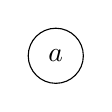
\begin{tikzpicture}
  \ARSnode{a};
\end{tikzpicture}

Normal forms: $a$. Terminating: True. Confluent: True. Unique NFs: True.

\subsection*{3.\; $A=\{a\},\; R=\{(a,a)\}$}
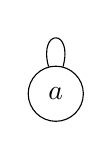
\begin{tikzpicture}
  \ARSnode{a};
  \path (a) edge[loop above] (a);
\end{tikzpicture}

Infinite $a\to a\to\cdots$: Terminating: \textbf{False}. Confluent: \textbf{True}. Unique NFs: \textbf{False}.

\subsection*{4.\; $A=\{a,b,c\},\; R=\{(a,b),(a,c)\}$}
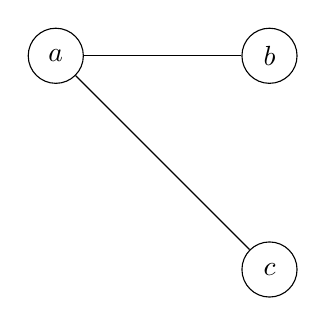
\begin{tikzpicture}[node distance=20mm]
  \ARSnode{a};
  \ARSnodeat{b}{right=of a}
  \ARSnodeat{c}{below=of b}
  \draw (a) edge (b) (a) edge (c);
\end{tikzpicture}

$b,c$ are normal; from $a$ you can reach two distinct NFs. Terminating: \textbf{True}. Confluent: \textbf{False}. Unique NFs: \textbf{False}.

\subsection*{5.\; $A=\{a,b\},\; R=\{(a,a),(a,b)\}$}
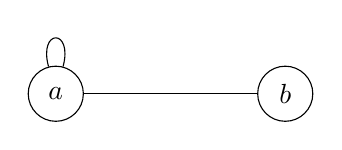
\begin{tikzpicture}[node distance=22mm]
  \ARSnode{a};
  \ARSnodeat{b}{right=of a}
  \draw (a) edge[loop above] (a) (a) edge (b);
\end{tikzpicture}

$b$ is normal; every element has the (unique) NF $b$. Terminating: \textbf{False}. Confluent: \textbf{True}. Unique NFs: \textbf{True}.

\subsection*{6.\; $A=\{a,b,c\},\; R=\{(a,b),(b,b),(a,c)\}$}
\begin{tikzpicture}[node distance=22mm]
  \ARSnode{a};
  \ARSnodeat{b}{right=of a}
  \ARSnodeat{c}{below=of b}
  \draw (a) edge (b) (a) edge (c) (b) edge[loop above] (b);
\end{tikzpicture}

Non-terminating via $b\to b$; $c$ is normal, $b$ has no NF. Confluent: \textbf{False}. Terminating: \textbf{False}. Unique NFs: \textbf{False}.

\subsection*{7.\; $A=\{a,b,c\},\; R=\{(a,b),(b,b),(a,c),(c,c)\}$}
\begin{tikzpicture}[node distance=22mm]
  \ARSnode{a};
  \ARSnodeat{b}{right=of a}
  \ARSnodeat{c}{below=of b}
  \draw (a) edge (b) (a) edge (c) (b) edge[loop above] (b) (c) edge[loop right] (c);
\end{tikzpicture}

Both $b$ and $c$ loop; no NFs reachable from $a$. Terminating: \textbf{False}. Confluent: \textbf{False}. Unique NFs: \textbf{False}.

\bigskip
\section*{Summary Table}
\begin{tabular}{@{}clccc@{}}
\toprule
\# & $(A,R)$ & confluent & terminating & has unique normal forms \\
\midrule
1 & $(\varnothing,\varnothing)$ & True & True & True \\
2 & $(\{a\},\varnothing)$ & True & True & True \\
3 & $(\{a\},\{(a,a)\})$ & True & False & False \\
4 & $(\{a,b,c\},\{(a,b),(a,c)\})$ & False & True & False \\
5 & $(\{a,b\},\{(a,a),(a,b)\})$ & True & False & True \\
6 & $(\{a,b,c\},\{(a,b),(b,b),(a,c)\})$ & False & False & False \\
7 & $(\{a,b,c\},\{(a,b),(b,b),(a,c),(c,c)\})$ & False & False & False \\
\bottomrule
\end{tabular}

\bigskip
\section*{All 8 combinations}
\begin{tabular}{@{}ccccl@{}}
\toprule
confluent & terminating & has unique NFs & example \\
\midrule
True  & True  & True  & e.g.\ ARS 2 (or 1) \\
True  & True  & False & \textit{Impossible} \\
True  & False & True  & ARS 5 \\
True  & False & False & ARS 3 \\
False & True  & True  & \textit{Impossible} \\
False & True  & False & ARS 4 \\
False & False & True  & \textit{Impossible} \\
False & False & False & ARS 6 (or 7) \\
\bottomrule
\end{tabular}

\end{document}
